\chapter{Darstellung der DICOM-Elemente im Speicher} \label{appendix:speicher}
\addthumb{Darstellung der DICOM-Elemente im Speicher}{\huge{\textbf{\thechapter}}}{white}{haw_rot}

\section{Explizite VR mit [ OB \textpipe\ OW \textpipe\ OF \textpipe\ SQ \textpipe\ UT \textpipe\ UN ]}

Bei expliziter VR-Struktur besteht das Element aus vier konsekutiven Feldern. Ist die VR vom Typ OB, OW, OF, SQ, UT oder UN wird das Datenelement wie in Tabelle \ref{table:appendix_explizit} im Speicher abgelegt. Die reservierten 2 Byte im VR-Teil sind für zukünftige Weiterentwicklungen des DICOM-Standards.\cite[7.1.2]{dicom:structure}

\begin{sidewaystable}
    \begin{tabularx}{\textwidth}{|X|X|p{4cm}|X|X|p{8cm}|}
    \toprule \hline
   \multicolumn{2}{|l|}{\textbf{Tag}} 	&	\multicolumn{2}{l|}{\textbf{VR}} 		&		\textbf{Value Length}   	& 	\textbf{Value} \\ \hline
    Group\# 16-bit unsigned integer & Element\# 16-bit unsigned integer  &  VR 2-byte character String [OB | OW | OF | SQ | UT | UN ] & Reservierter
    Bereich & 32-bit unsigned integer  &  Gerade Anzahl an Byte. Enthält den Wert des Datenelements. Kodierung abhängig von VT-Typ und Transfersyntax. Wenn die Länge nicht definiert ist, wird diese auf \glqq Sequence Delimitation\grqq\ limitiert. \\ \hline
	
	2 Byte & 2 Byte & 2 Byte & 2 Byte & 4 Byte & Anzahl an Byte entsprechend der \glqq Value Length\grqq\, wenn von expliziter Länge \\ \hline
	
	\bottomrule
    \end{tabularx}
    \caption {Darstellung des Datenelements im Speicher wenn VR vom Typ OB, OW, OF, SQ, UT oder UN}
    \label{table:appendix_explizit}
\end{sidewaystable}

\section{Explizite VR}

Diese Darstellung wird gewählt, wenn VR \textit{nicht} vom Typ OB, OW, OF, SQ, UT oder UN ist. Der Unterschied besteht im Feld \glqq Value Length\grqq. Bei der Form von Tabelle \ref{table:appendix_explizit} ist dieses Feld 32 Bit lang. Hier beträgt es lediglich 16 Bit \cite[7.1.2]{dicom:structure}. Der Grund liegt am erhöhten Speicherbedarf von \ref{table:appendix_explizit}, da die Länge des Wertes eine undefinierte Länge haben kann.

\begin{sidewaystable}
	\begin{tabularx}{\textwidth}{|X|X|X|X|p{12cm}|}
	\toprule \hline
	\multicolumn{2}{|l|}{\textbf{Tag}} & \textbf{VR} 2 & \textbf{Value Length} & \textbf{Value} 4 \\ \hline
	Group\# 16-bit unsigned integer & Element\# 16-bit unsigned integer & VR 2-byte character String 2 & 16-bit unsigned integer & Gerade Anzahl an Byte. Enthält den Wert des Datenelements. Kodierung abhängig von VT-Typ und Transfersyntax. \\ \hline
	2 Byte & 2 Byte & 2 Byte & 2 Byte & \glqq Value Length\grqq\ Byte \\ \hline
	\bottomrule
	\end{tabularx}
    \caption {Darstellung des Datenelements für alle anderen VR-Typen}
    \label{table:appendix_explizit_else}
\end{sidewaystable}

\section{Implizite VR}

Bei einer impliziten VR Darstellung besteht das Datenelement aus den drei konsekutiven Feldern Tag, Value Length und dem Wert selbst \cite[7.1.3]{dicom:structure}.

\begin{sidewaystable}
	\begin{tabularx}{\textwidth}{|X|X|X|p{12cm}|}
	\toprule \hline
	\multicolumn{2}{|l|}{\textbf{Tag}} & \textbf{Value Length} 2 & \textbf{Value} \\ \hline
	Group\# 16-bit unsigned integer & Element\# 16-bit unsigned integer & 32-bit unsigned integer & Gerade Anzahl an Byte. Enthält den Wert des Datenelements. Kodierung abhängig von VT-Typ spezifiziert in \cite{dicom:dd} und Transfersyntax. Wenn die Länge nicht definiert ist wird diese auf \glqq Sequence Delimitation\grqq\ limitiert. \\ \hline
	2 Byte & 2 Byte & 2 Byte & \glqq Value Length\grqq\ Byte oder undefinierte Länge \\ \hline
	
	\bottomrule
	
	\end{tabularx}
    \caption {Darstellung des Datenelements für implizite VR.}
    \label{table:appendix_implizit}
\end{sidewaystable}


\chapter{Installation der Eclipse e4 Umgebung} \label{install_eclipse}
\addthumb{Installation der Eclipse e4 Umgebung}{\huge{\textbf{\thechapter}}}{white}{haw_rot}
\section{Eclipse}
Voraussetzung für Eclipse ist eine bereits installierte Java Virtual Machine. Werden keine Werkzeuge aus dem Java Development Kit benötigt, reicht eine Java Runtime Environment aus. Für die Entwicklung von jMediKit wurde Java 7 verwendet.\\
Grundlage für die Plug-in und Rich Client Entwicklung ist eine Eclipse-Installation ab Version 4. Unter \textit{http://www.eclipse.org/downloads/} kann der aktuelle \textit{Eclipse Standard Client} für ein beliebiges Betriebssystem bezogen werden. Bei der Wahl zwischen 32- und 64-Bit muss die Version mit der installierten Java-Variante übereinstimmen, da sonst die Native Libraries nicht geladen werden können. Nach dem Entpacken des Zip-Archivs kann der Client über \textit{eclipse.exe} gestartet werden. Abbildung \ref{eclipsestd} zeigt das Programmfenster von Eclipse nach dem ersten Ausführen.\\

\begin{figure}[H]
  \vspace{0.5cm}
  \centering
  \fbox{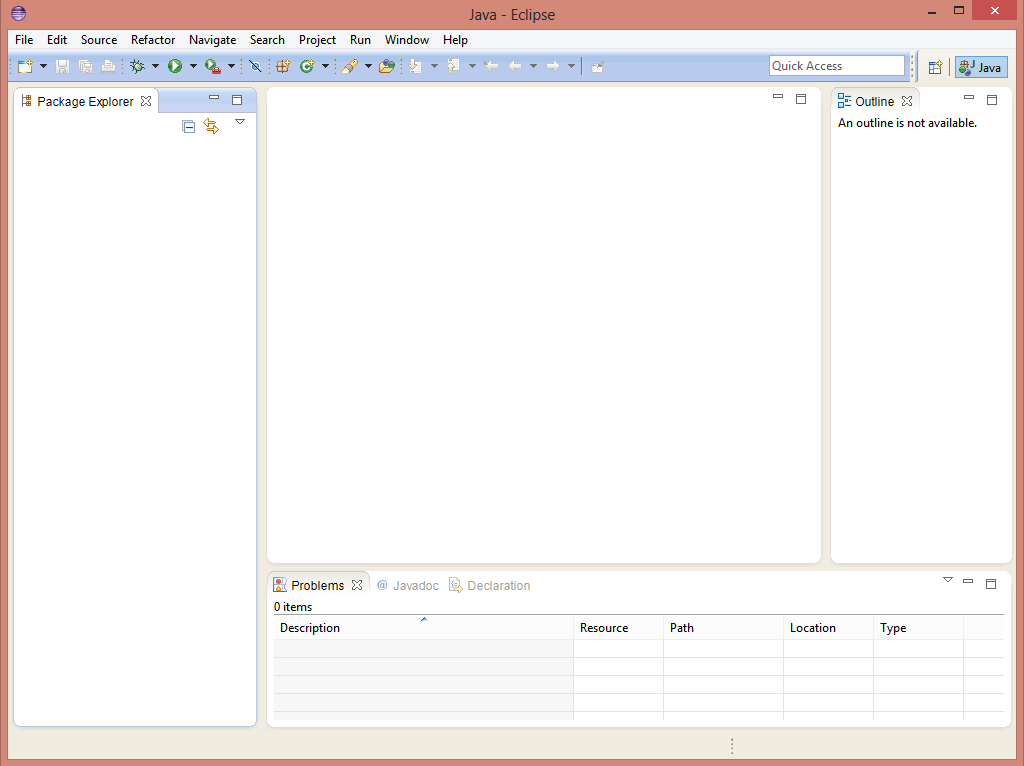
\includegraphics[angle=0,width=8cm]{./img/eclipse_std.png}}
  \caption{Standardinstallation eines 32-Bit Eclipse unter Windows 8}
  \label{eclipsestd}
  \vspace{0.5cm}
\end{figure}

\section{Eclipse e4 Tools}
Eine weitere Voraussetzung ist eine Installation der e4 Tools. Das e4 Projekt ist unter \textit{http://download.eclipse.org/e4/downloads/} mit dem Punkt \textit{Stable Build} zu finden (Abbildung \ref{e4download}). 

\begin{figure}[H]
  \vspace{0.5cm}
  \centering
  \fbox{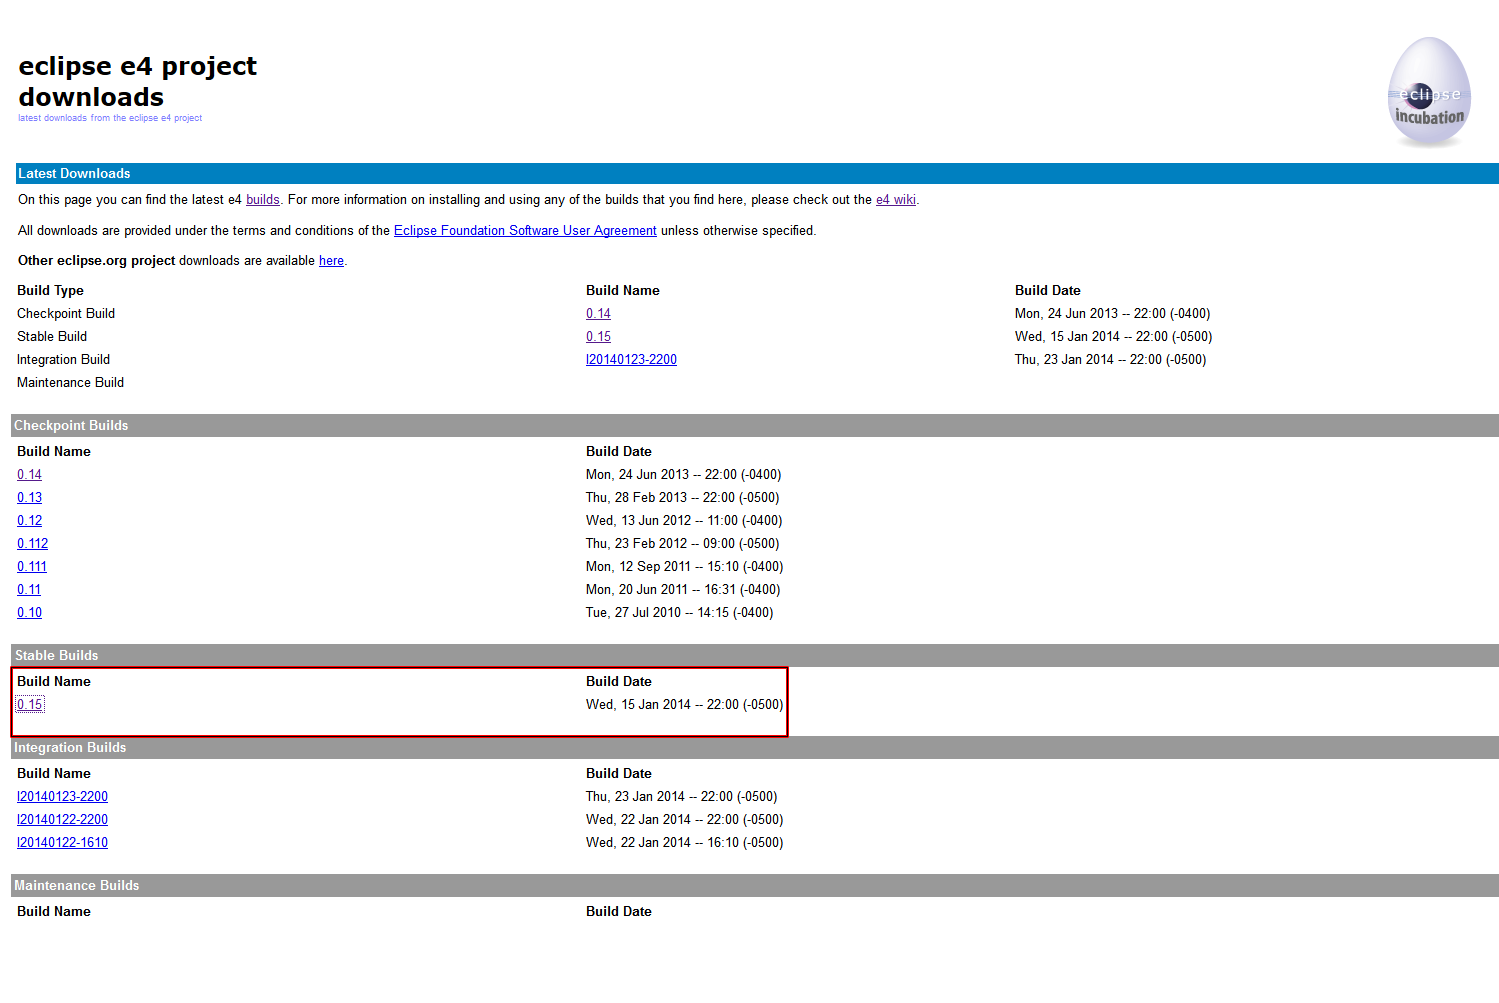
\includegraphics[angle=0,width=8cm]{./img/e4download.png}}
  \caption{e4 Projekt Builds}
  \label{e4download}
  \vspace{0.5cm}
\end{figure}

Nach einem Klick auf den aktuellen Build öffnet sich die Seite mit dem Link zum Repository wie in Abbildung \ref{repolink} rot markiert.\\
Dieser Link (\textit{http://download.eclipse.org/ e4/ downloads/ drops/ S-0.15-201401152200/ repository} - Stand 24.01.2014) muss nun in die Zwischenablage kopiert werden.

\begin{figure}[H]
  \vspace{0.5cm}
  \centering
  \fbox{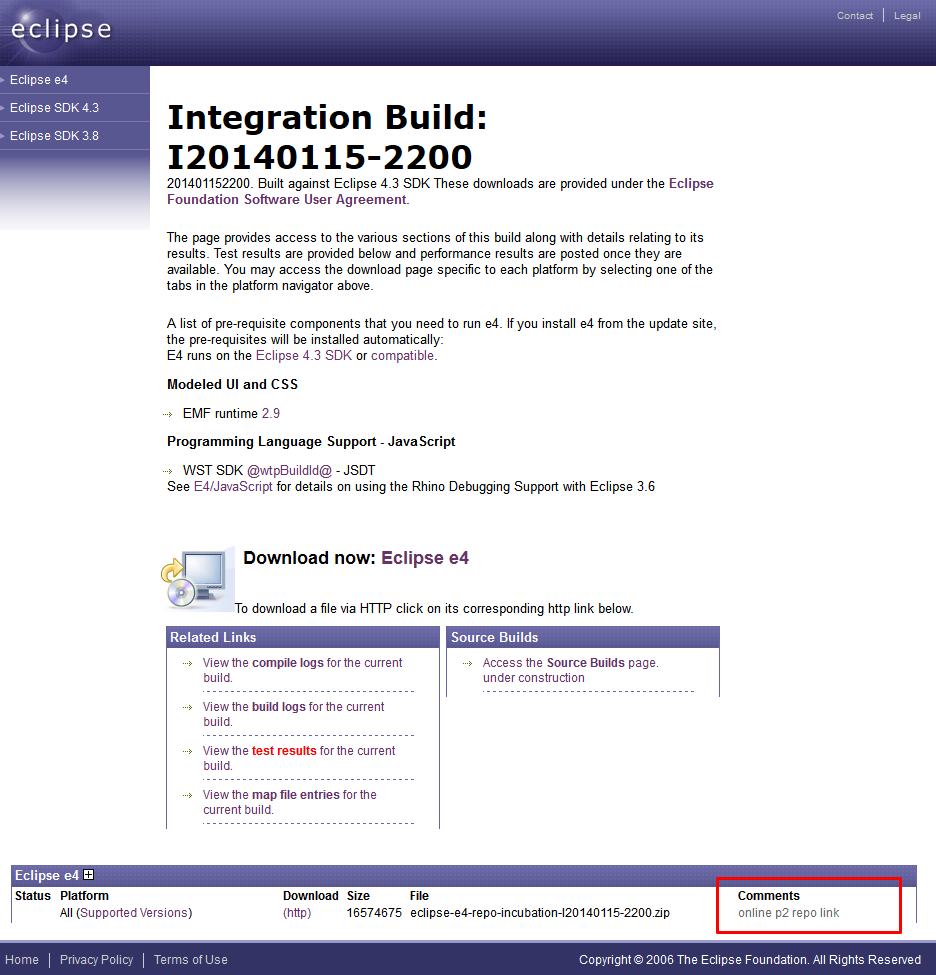
\includegraphics[angle=0,width=8cm]{./img/repolink.png}}
  \caption{e4 Repository Link}
  \label{repolink}
  \vspace{0.5cm}
\end{figure}

Nachdem der Link kopiert wurde, kann Eclipse geöffnet werden. Nach einem Klick auf den Menüpunkt \textit{Hilfe} $\rightarrow$ \textit{Install New Software} öffnet sich ein Fenster mit dem Titel \glqq Available Software\grqq\ wie in Abbildung \ref{installnew} zu sehen ist. 

\begin{figure}[H]
  \vspace{0.5cm}
  \centering
  \fbox{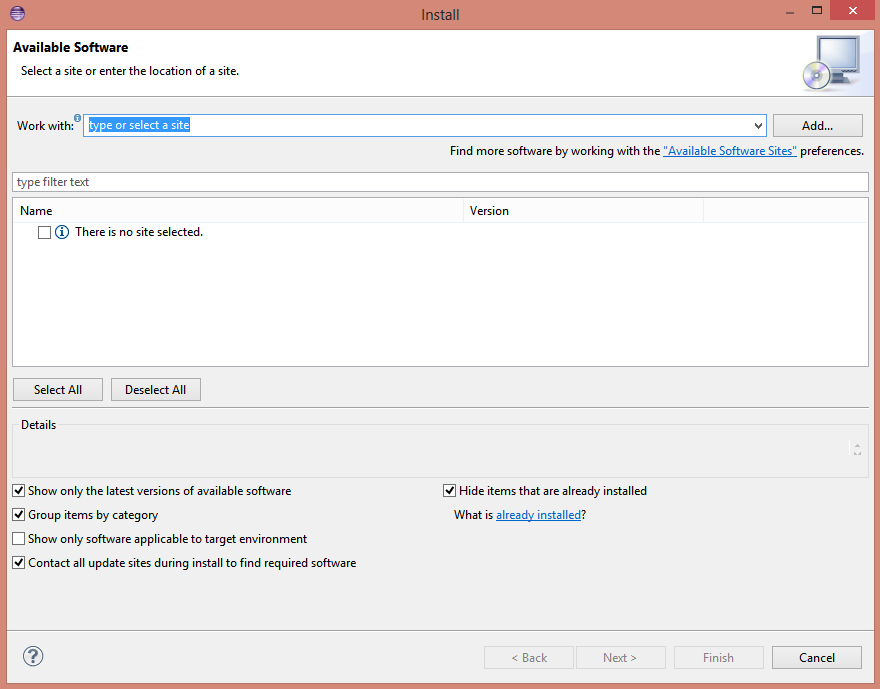
\includegraphics[angle=0,width=8cm]{./img/installnew.png}}
  \caption{Installation neuer Software unter Eclipse}
  \label{installnew}
  \vspace{0.5cm}
\end{figure}

Mit dem Button \textit{Add} wird nun der zuvor kopierte Link als Repository angegeben. Der \textit{Name} kann frei vergeben werden. Unter \textit{Location} muss man den Link zum Repository eintragen. Danach mittels \textit{OK} die Aktion bestätigen.

\begin{figure}[H]
  \vspace{0.5cm}
  \centering
  \fbox{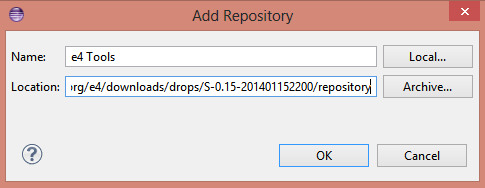
\includegraphics[angle=0,width=6cm]{./img/insertrepo.png}}
  \caption{Angabe des Repository}
  \label{insertrepo}
  \vspace{0.5cm}
\end{figure}

Nach einem korrekten Eintrag wird die Liste der verfügbaren Software, wie in Abbildung \ref{e4install} zu sehen ist, aktualisiert. Hier muss das Paket \textit{Eclipse 4 core tools} samt Unterpakete ausgewählt werden. Mit einem Klick auf \textit{Next} startet die Installationsroutine. Hierbei ist den Anweisungen auf dem Bildschirm zu folgen. Nach einer erfolgreichen Installation muss Eclipse neu gestartet werden.

\begin{figure}[H]
  \vspace{0.5cm}
  \centering
  \fbox{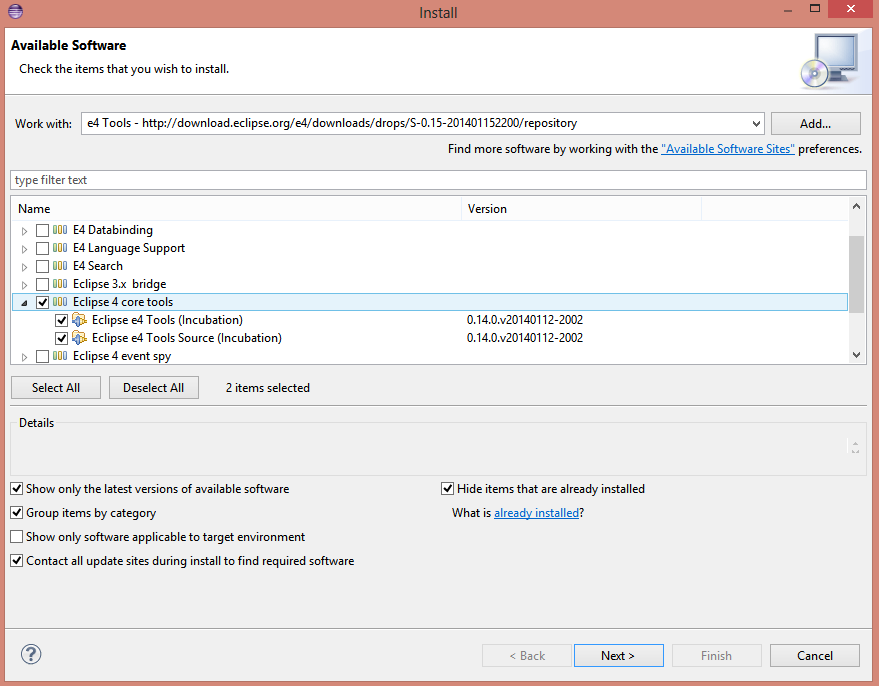
\includegraphics[angle=0,width=8cm]{./img/e4install.png}}
  \caption{Auswahl der e4 Tools zur Installation}
  \label{e4install}
  \vspace{0.5cm}
\end{figure}

\section{Import der jMediKit Projektdateien}

Die Projektdaten befinden sich auf dem beiliegenden Datenträger. Das Wurzelverzeichnis kann als Eclipse Workspace benutzt werden. Dabei ist darauf zu achten, dass der Ordner \textit{/.metadata/.plugins} leer ist. Sollten sich Daten darin befinden, können diese gelöscht werden. Eclipse erstellt bei Bedarf die Plug-in-Daten neu. Der Workspace besteht aus den drei Projekten \textit{org.jmedikit.product}, \textit{org.jmedikit.feature} und \textit{org.jmedikit.plugin}. Beim ersten Öffnen ist der Package Explorer leer und die Projekte müssen importiert werden. Nach einem Klick auf \textit{File} $\rightarrow$ \textit{Import} erscheint ein Dialog wie in Abbildung \ref{importproject} zu sehen ist. Bei der Auswahl muss der Punkt unter \textit{General} $\rightarrow$ \textit{Existing Projects into Workspace} markiert und mit \textit{Next} bestätigt werden. Im folgenden Fenster (Abbildung \ref{selectimport}) muss unter ausgewähltem \textit{Select Root Directory} unter \textit{Browse} das Wurzelverzeichnis von jMediKit angegeben werden. Danach können die verfügbaren Projekte hinzugefügt und mittels Klick auf \textit{Finish} in den Eclipse Workspace importiert werden.

\begin{figure}[H]
%\subfigure[Keypoints]{\includegraphics[width=0.49\textwidth]{./img/basmati_keypoints.png}}\hfill
\centering
\fbox{
\subfigure[Dialog zum Import von Eclipse-Projekten]{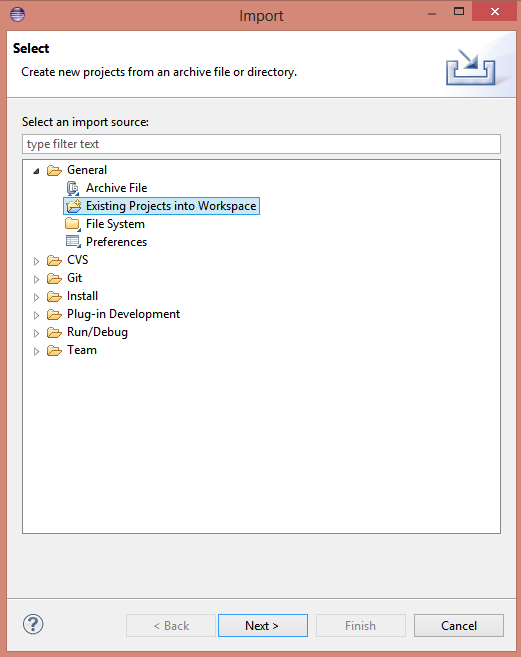
\includegraphics[width=6cm]{./img/import.png} \label{importproject}}
\subfigure[Auswahl der Projekte]{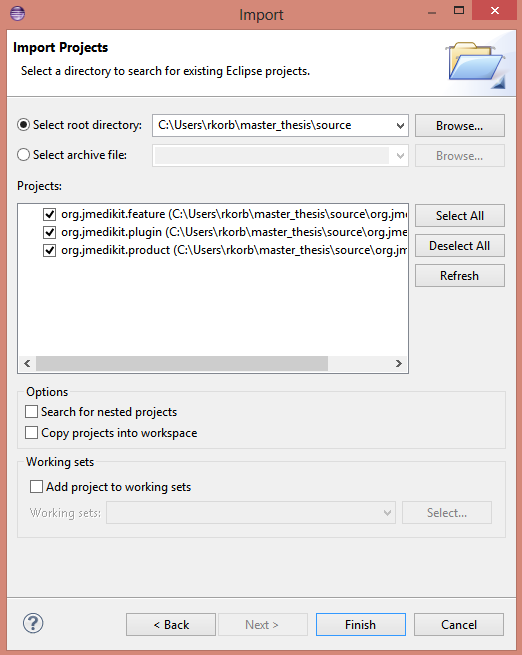
\includegraphics[width=6cm]{./img/importprojects.png} \label{selectimport}}
}
\caption{Vorgang zum Importieren bereits bestehender Projekte}
\label{import}
\end{figure}

War der Importvorgang erfolgreich, sind die drei Projekte 

\begin{itemize}
\item \textit{org.jmedikit.product}
\item \textit{org.jmedikit.feature}
\item  \textit{org.jmedikit.plugin} 
\end{itemize}

wie in Abbildung \ref{finishedimport} zu sehen, im Package Explorer vorhanden.

\begin{figure}[H]
  \vspace{0.5cm}
  \centering
  \fbox{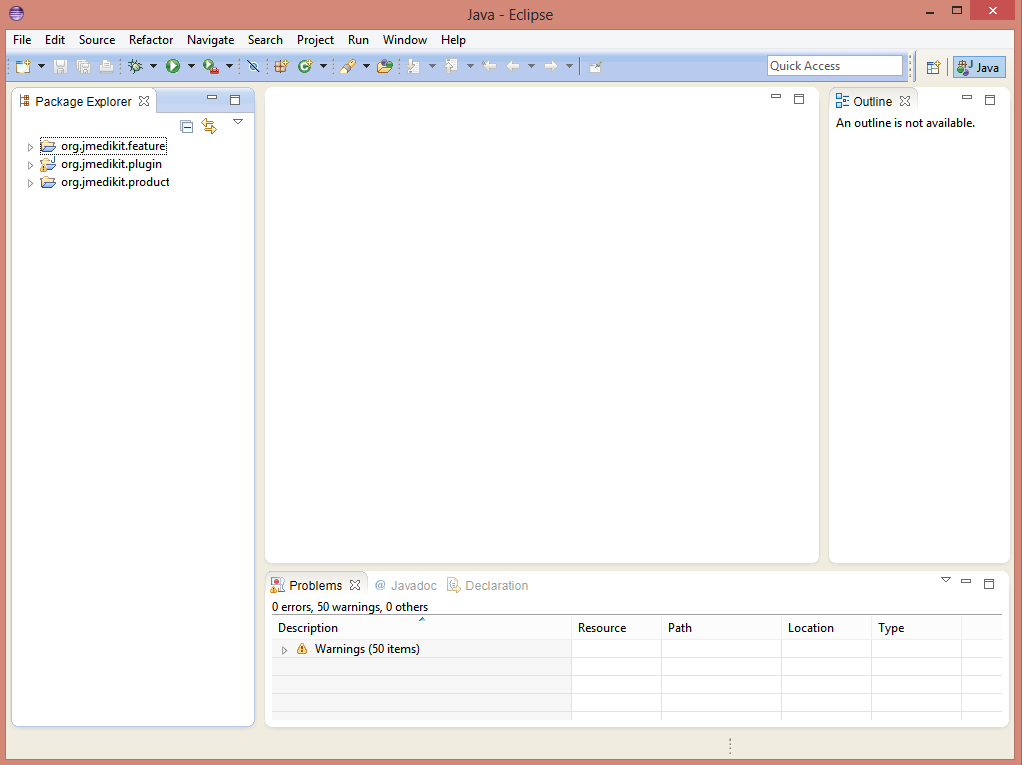
\includegraphics[angle=0,width=8cm]{./img/imported.png}}
  \caption{Der Package Explorer nach dem Importvorgang}
  \label{finishedimport}
  \vspace{0.5cm}
\end{figure}

Im Projekt \textit{org.jmedikit.product} befindet sich die Datei \textit{jmedikit.product}. Nach einem Doppelklick wird die Datei im Eclipse-Editor geöffnet und zeigt die Grundlegende Anwedungsdefinition von jMediKit und den zugehörigen Einstellungen. Unter dem Tab \textit{Overview} im Bereich \textit{Test} kann jMediKit mit einem Klick auf \textit{Launch an Eclipse application} gestartet werden. Abbildung \ref{launchjmedikit} hebt die Schaltfläche hervor. Bei einem ersten Start wird jMediKit mit einer Fehlermeldung geschlossen, da von Eclipse noch nicht alle zum Start notwendigen Plug-ins geladen wurden, welche von jMediKit benötigt werden.

\begin{figure}[H]
  \vspace{0.5cm}
  \centering
  \fbox{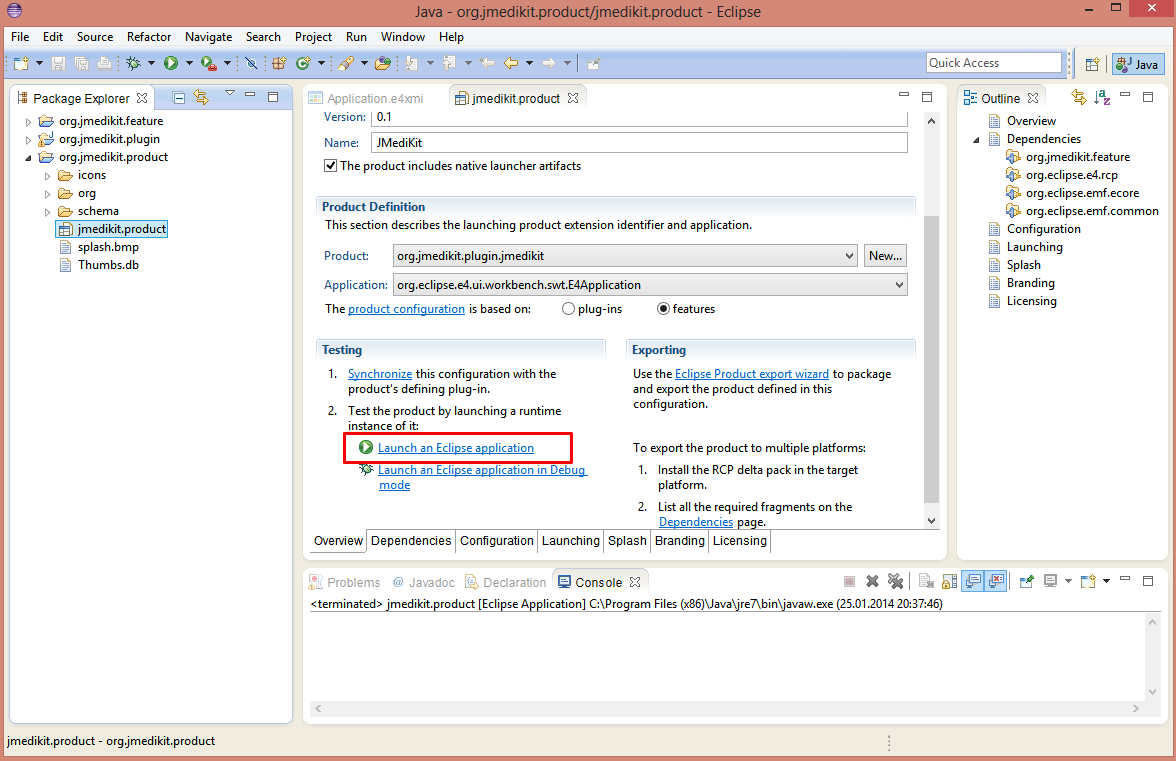
\includegraphics[angle=0,width=8cm]{./img/launch.png}}
  \caption{Der Package Explorer nach dem Importvorgang}
  \label{launchjmedikit}
  \vspace{0.5cm}
\end{figure}

Unter \textit{Run} $\rightarrow$ \textit{Run Configuration} können die Plug-ins zur Verfügung gestellt werden. Abbildung \ref{addplugins} zeigt das Konfigurationsfenster. Im linken Teil muss die Product-Datei jmedikit.product ausgewählt sein. Unter dem Tab \textit{Plug-ins} befindet sich auf der rechten Seite die Schaltfläche \textit{Add Required Plug-ins}. Nach einem Klick auf \textit{Apply} gefolgt von \textit{Run} kann jMediKit gestartet werden.

\begin{figure}[H]
  \vspace{0.5cm}
  \centering
  \fbox{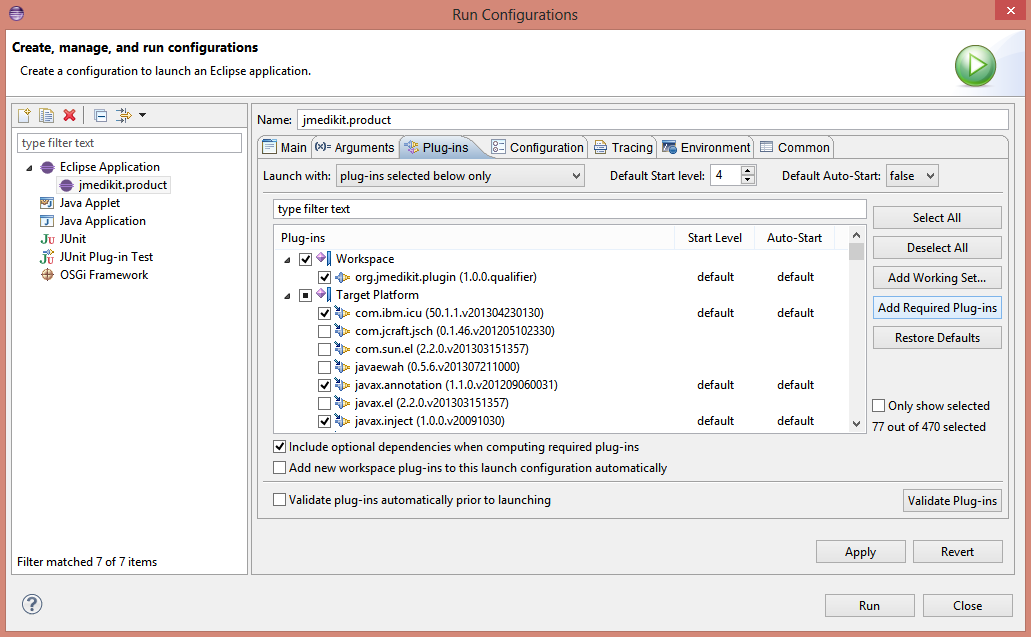
\includegraphics[angle=0,width=8cm]{./img/addplugins.png}}
  \caption{Konfigurationsfenster zu Anwendungseinstellungen und Anwendungsstart}
  \label{addplugins}
  \vspace{0.5cm}
\end{figure}

\section{Installation des Java Advanced Imaging Image I/O Tools}
jMediKit benutzt die externe Bibliothek \glqq dcm4che\grqq, um DICOM-Objekte zu laden und die Bilder auf der Zeichenfläche anzuzeigen. \glqq dcm4che\grqq\ selbst benötigt das Paket \glqq Java Advanced Imaging Image I/O Tools\grqq. Ist das Tool noch nicht installiert, kann unter der Adresse \textit{http://download.java.net/media/jai-imageio/builds/release/1.1/}, entsprechend dem Betriebssystem und der Installationsart, die richtige Version zum Installieren gewählt werden. Ob der JDK- oder JRE-Installationstyp verwendet werden soll, hängt von der in Eclipse verwendeten Java Runtime Environment ab. Ist eine eigenständige JRE istalliert, hat diese beispielsweise den Pfad \textit{/JAVA\_HOME/jre7/} und es wird die JRE-Variante installiert. Hat die JRE zum Beispiel einen Pfad der Form \textit{/JAVA\_HOME/ jdk1.7.0\_45/jre} ist die Java Runtime Environment des Java Development Kits im Einsatz.\\
Um zu prüfen, welche Java Runtime Environment von Eclipse verwendet wird, muss der Einstellungsdialog unter \textit{Window} $\rightarrow$ \textit{Preferences} geöffnet und der Punkt \textit{Java} $\rightarrow$ \textit{Installed JREs} gewählt werden. Abbildung \ref{jai} zeigt den Dialog mit einer JRE und dem Pfad C:$\backslash$Program Files (x86)$\backslash$Java$\backslash$jre7.
\begin{figure}[H]
  \vspace{0.5cm}
  \centering
  \fbox{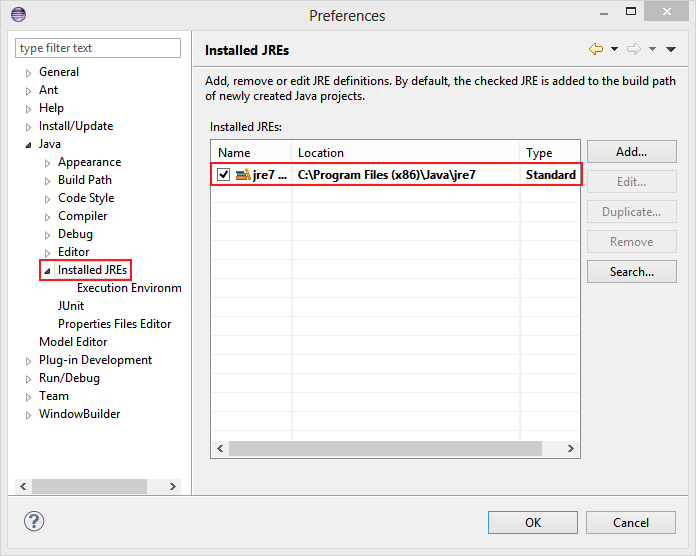
\includegraphics[angle=0,width=8cm]{./img/jaiimageio.png}}
  \caption{Die von Eclipse verwendeten Java Runtime Environments}
  \label{jai}
  \vspace{0.5cm}
\end{figure}

Ob die Image I/O Tools installiert sind, kann über den Ordner der externen Bibliotheken der Java-Installation geprüft werden. Sind im Ordner \textit{/PATH\_TO\_JRE/lib/ext/} die .jar-Pakete \textit{jai\_imageio} und \textit{clibwrapper\_jiio} vorhanden, kann \glqq dcm4che\grqq\ auf die Bibliothek zugreifen.\\
Die Java Advanced Imaging Image I/O Tools sind nur in einer 32-Bit Version verfügbar. Bei einer Installation werden native Bibliotheken in die JRE integriert. Werden die Tools mit einer 64-Bit Java und Eclipse Version eingesetzt, sind diese nativen Bibliotheken nicht verfügbar.
Eine Installation für eine 64-Bit JRE erfolgt über das Verschieben der .jar-Dateien \textit{jai\_imageio} und \textit{clibwrapper\_jiio} in das Verzeichnis \textit{/PATH\_TO\_x64JRE/lib/ext/} der 64-Bit JRE.\\
Durch das Fehlen des nativen Codes einer 64-Bit Installation können nicht alle DICOM-Bilder geladen werden, da zum Beispiel eine Komprimierung im Format \textit{JPEG2000} davon abhängig ist. 

\section{Erstellung eines neuen Builds von jMediKit}

Um einen neuen Build von jMediKit zu veröffentlichen, muss die Datei \textit{jmedikit.product} im Projekt \textit{org.jmedikit.product} mit einem Doppelklick geöffnet werden. Darauf öffnet sich der \textit{Overview} zum Produkt, wie in Abbildung \ref{build} zu sehen ist. Am oberen rechten Rand des \textit{Overviews} sind vier Buttons angeordnet. Hier muss der dritte Button names \textit{Export an Eclipse product}(in der Abbildung \ref{build} rot markiert) gedrückt werden.

\begin{figure}[H]
  \vspace{0.5cm}
  \centering
  \fbox{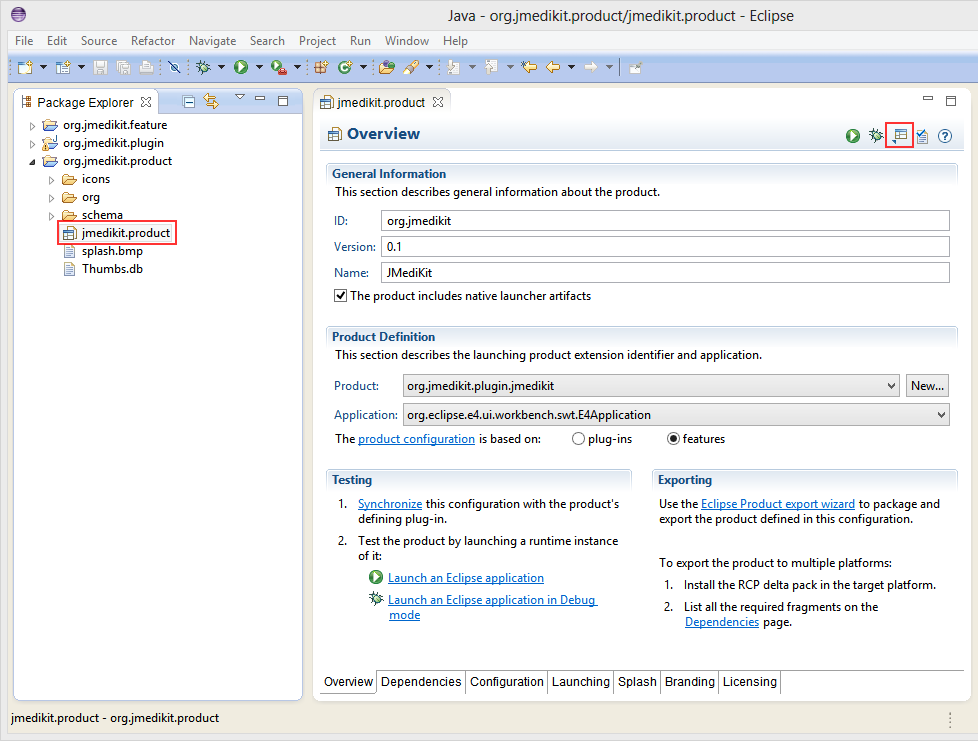
\includegraphics[angle=0,width=8cm]{./img/jmedikit_build.png}}
  \caption {Mit jmedikit.product den Build erstellen}
  \label{build}
  \vspace{0.5cm}
\end{figure}

Es öffnet sich ein Fenster mit diversen Optionen(Abbildung \ref{buildoptions}).Als \textit{Configuration} muss die \textit{jmedikit.product} gewählt werden. Unter \textit{Root Directory} wird das Wurzelverzeichnis von jMediKit bestimmt. Die Option \textit{Directory} ist das Exportverzeichnis, in dem die Anwendung nach dem Build zu finden ist. Die weiteren Optionen entsprechen der Abbildung \ref{buildoptions}. Mit \textit{Finish} wird der Build-Prozess gestartet.

\begin{figure}[H]
  \vspace{0.5cm}
  \centering
  \fbox{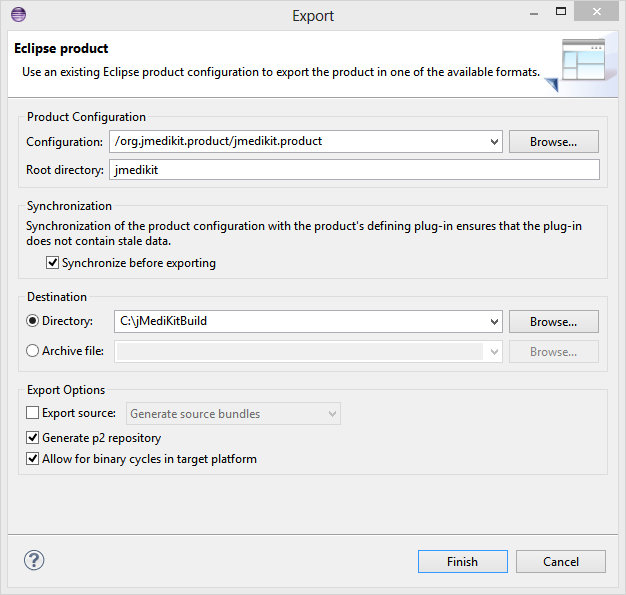
\includegraphics[angle=0,width=8cm]{./img/jmedikit_buildoptions.png}}
  \caption {Optionen zur Erstellung des Builds}
  \label{buildoptions}
  \vspace{0.5cm}
\end{figure}

\chapter{Iconverwaltung innerhalb der Anwendung} \label{importicon}
\addthumb{Iconverwaltung innerhalb der Anwendung}{\huge{\textbf{\thechapter}}}{white}{haw_rot}

Die Icons der Anwendung werden mit Hilfe eines OSGi-Services verwaltet. Eclipse definiert das Interface \textit{IResourceProviderService}, mit dessen Hilfe die Bilddaten organisiert werden können. Die Metadaten des Services befinden sich im Projekt \textit{org.jmedikit.plugin} unter \textit{OSGI-INF}. Hier wird der spezifische Service bekannt gemacht und die implementierende Klasse festgelegt. Zusätzlich wird die Datei \textit{OSGI-INF/resource.properties} definiert, die alle Pfadangaben zu den Bilddateien enthält.\\
Um neue Bilder und Icons hinzuzufügen muss zuerst die Datei \textit{resource.properties} um einen Bezeichner und die Pfadangabe erweitert werden. Ein neuer Eintrag kann an beliebiger Stelle, wie in Listing \ref{resource}, hinzugefügt werden.

\lstset{
language=sh,
caption={resource.properties},
label=resource,
xleftmargin=1em,
xrightmargin=1em,
numbers=left,
backgroundcolor=\color{lgrey},
}  
\begin{figure}[htbp]
\begin{lstlisting}[frame=leftline]
NEW_ICON_FILE=icons/mynewicon.png
\end{lstlisting}

\end{figure}

Der \textit{ImageProvider} erweitert die von Eclipse bereitgestellte Klasse \textit{BasicImageProvider}, die das Interface des Services implementiert. \textit{ImageProvider} muss nun um den Bezeichner des neuen Icons mit einer Konstanten erweitert werden (Listing \ref{konst}).

\lstset{
language=Java,
caption={Erweiternder Eintrag einer Konstanten in der Klasse \textit{ImageProvider}},
label=konst,
xleftmargin=1em,
xrightmargin=1em,
numbers=left,
backgroundcolor=\color{lgrey},
}  
\begin{figure}[htbp]
\begin{lstlisting}[frame=leftline]
public final static String NEW_ICON_FILE = "NEW_ICON_FILE";
\end{lstlisting}

\end{figure}

Die Bilddatei oder das Icon wird nach einem erneuten Build des Services verfügbar. Dieser kann zum Beispiel durch ein erneutes Speichern der Datei \textit{org.jmedikit.plugin/META-INF/MANIFEST.MF} angestoßen werden.
Listing \ref{use} zeigt die Verwendung der neuen Bilder und Icons. Innerhalb der Klassen, die Strukturen des Application Models implementieren, kann mit der in Eclipse e4 verfügbaren \textit{Dependency Injection} gearbeitet werden\footnote{Ein umfassender Artikel zur Dependency Injection ist unter \cite{vogel:di} verfügbar.}. Existiert innerhalb des Lebenszyklus der Anwendung ein \textit{IResourcePool}-Objekt, kann es mit Hilfe der Annotation \textit{@Inject} in die Klasse injiziert werden. Mit dieser Instanz wird innerhalb der Anwendung ein SWT.Image mit der Methode \textit{getImageUnchecked} instantiiert.
\lstset{
language=Java,
caption={Verwendung des ImageProviders mit dem IResourcePool},
label=use,
xleftmargin=1em,
xrightmargin=1em,
numbers=left,
backgroundcolor=\color{lgrey},
}  
\begin{figure}[htbp]
\begin{lstlisting}[frame=leftline]
//Erzeugen eine SWT.Image aus dem ImageProvider
public class PartClass{

	/**
	 * Den IResourcePool mittels 
	 * Dependency Injection verfuegbar machen
	 */
	@Inject
	IResourcePool provider;
	
	public void someMethod(){
	 	Image icon = provider.getImageUnchecked(
			ImageProvider.NEW_ICON_FILE
	 	);
	}
}
\end{lstlisting}

\end{figure}

\chapter{Die Verwendung von Eclipse zur Plug-in-Entwicklung}
\addthumb{Die Verwendung von Eclipse zur Plug-in-Entwicklung}{\huge{\textbf{\thechapter}}}{white}{haw_rot}

Dieses Kapitel beschreibt das Vorbereiten eines Projekts zur Entwicklung eines Plug-ins für jMediKit. Voraussetzung für diese Anleitung ist Eclipse ab Version 4. Zusätzlich wird entweder ein Build von jMediKit oder der Quelltext und die im Plug-in verwendeten externen Bibliotheken benötigt.\\
Nachdem Eclipse geöffnet wurde, kann über \textit{File} $\rightarrow$ \textit{New} $\rightarrow$ \textit{Java Project} ein neues Javaprojekt angelegt werden. Abbildung \ref{newproject} zeigt den entsprechenden Dialog und die zu wählenden Eigenschaften. Es muss nur der Plug-in Name bestimmt werden. Die restlichen Einstellungen entsprechen den Standardwerten, können aber nach Bedarf angepasst werden.

\begin{figure}[H]
  \vspace{0.5cm}
  \centering
  \fbox{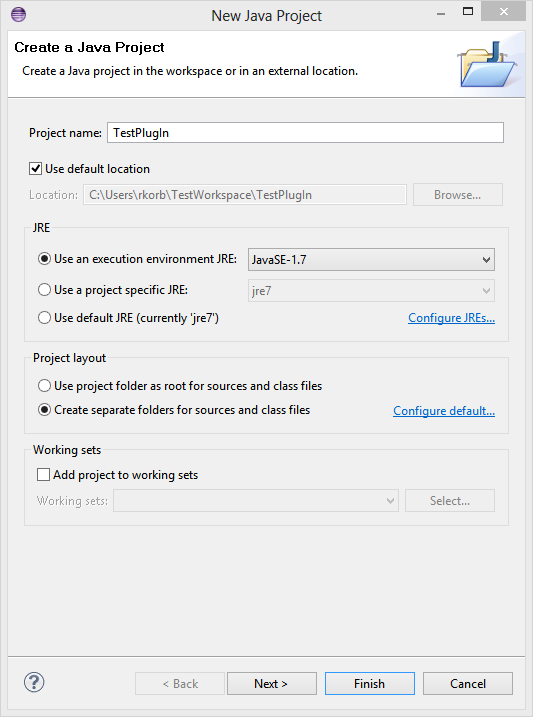
\includegraphics[angle=0,width=6cm]{./img/plugin_newprojekt.png}}
  \caption{Dialog zum Anlegen eines neuen Javaprojekts}
  \label{newproject}
  \vspace{0.5cm}
\end{figure}

Mit einem Klick auf \textit{Next} wird man zu den nächsten Projektoptionen, wie in Abbildung \ref{binfolder} zu sehen, geleitet. Hier kann unter \textit{Default Output Folder} der Ordner entsprechend der Plug-in-Konventionen für die \textit{.class} Dateien gesetzt werden. Der Plug-in-Name im Beispiel lautet \textit{TestPlugIn}. Entsprechend ist unter \textit{Default Output Folder} der Wert \mbox{\textit{TestPlugIn/\_\_TestPlugIn}} einzutragen, wobei \textit{TestPlugIn} den Projektordner darstellt und die Binärdaten unter \textit{\_\_TestPlugIn} gespeichert werden. Der Name des Output-Ordners für die Binärdaten kann später manuell in Eclipse mit einem \textit{Rechtsklick auf das Projekt} $\rightarrow$ \textit{Build Path} $\rightarrow$ \textit{Configure Build Path} $\rightarrow$ \textit{Unter dem Tab Source} $\rightarrow$ \textit{Default Output Folder} ausgelesen oder geändert werden.

\begin{figure}[H]
  \vspace{0.5cm}
  \centering
  \fbox{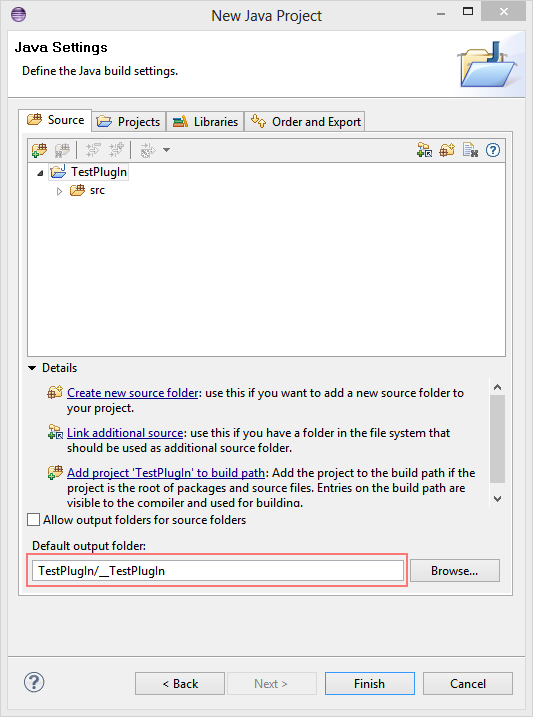
\includegraphics[angle=0,width=6cm]{./img/plugin_binfolder.png}}
  \caption{Auswahl des Output-Ordners}
  \label{binfolder}
  \vspace{0.5cm}
\end{figure}

Im nächsten Schritt müssen die externen Bibliotheken dem Projekt hinzugefügt werden. Werden vom User selbst keine speziellen Bibliotheken verwendet, reicht das Inkludieren der jMediKit-Bibliothek und dem SimpleITK-Projekt.\\
Dazu muss im aktuellen Dialogfenster der Reiter \textit{Libraries} ausgewählt werden. Wird mit einem jMediKit-Build gearbeitet, kann die Bibliothek mit dem Button \textit{Add External Jar} hinzugefügt werden. Nach einem Klick öffnet sich ein Dateidialog. Der Pfad zu der jMediKit-Jar befindet sich unter \newline
\textit{jMedikit-Installation/}\textit{jmedikit/}\textit{plugins/}\textit{org.jmedikit.plugin\_versionsnummer}, wobei \textit{versionsnummer} für die Versionsnummer des aktuellen Builds steht(zum Beispiel\newline \textit{org.jmedikit.plugin\_1.0.0.201401220023}). Wird mit dem Quelltext von jMediKit gearbeitet, können die Projektdateien über den Button \textit{Add External Class Folder} hinzugefügt werden. Diese liegen im Ordner \textit{bin} im Projekt \textit{org.jmedikit.plugin}. Der Vollständige Pfad ist \textit{/WORKSPACE/org.jmedikit.plugin/bin/}.\\
Um die SimpleITK.jar einzubinden gibt es zwei Möglichkeiten. Wird mit dem Build gearbeitet, kann die jMediKit-Jar mit einem Zip-Programm geöffnet und SimpleITK aus dem Ordner \textit{lib} entpackt werden\footnote{Ist kein Programm zum Entpacken von jar-Dateien vorhanden, kann SimpleITK direkt von \textit{http://www.simpleitk.org/SimpleITK/resources/software.html} bezogen werden}. Bei der Verwendung der Quelldateien liegt die Bibliothek von SimpleITK im Projekt \textit{org.jmedikit.plugin} ebenfalls im Ordner \textit{lib} mit dem vollständigen Pfad \textit{/WORKSPACE/org.jmedikit.plugin/lib/SimpleITK/}. Die Datei \textit{simpleitk-0.x.x.jar} kann nun mit dem Button \textit{Add External Jar} hinzugefügt werden.

\begin{figure}[H]
  \vspace{0.5cm}
  \centering
  \fbox{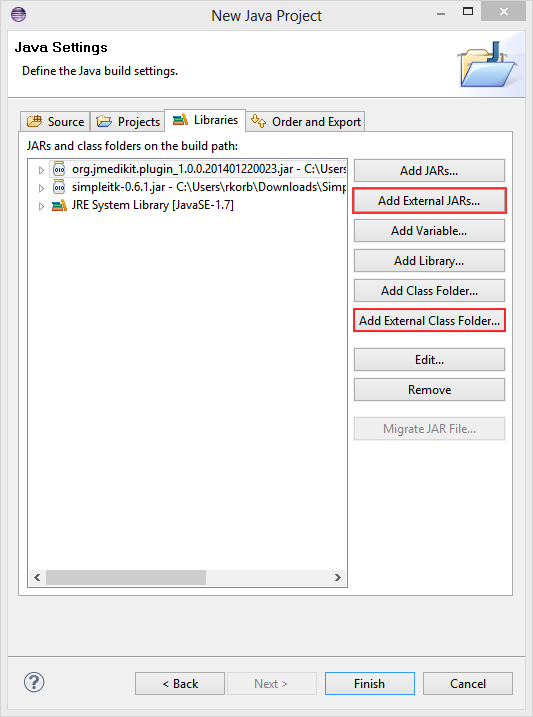
\includegraphics[angle=0,width=6cm]{./img/plugin_libs.png}}
  \caption{Auswahl der externen Bibliotheken}
  \label{libs}
  \vspace{0.5cm}
\end{figure}

Mit einem Klick auf \textit{Finish} werden die Einstellungen übernommen und das Projekt angelegt. Wurden alle Schritte korrekt ausgeführt, hat das Plug-in-Projekt eine Struktur wie in Abbildung \ref{workspace}.

\begin{figure}[H]
  \vspace{0.5cm}
  \centering
  \fbox{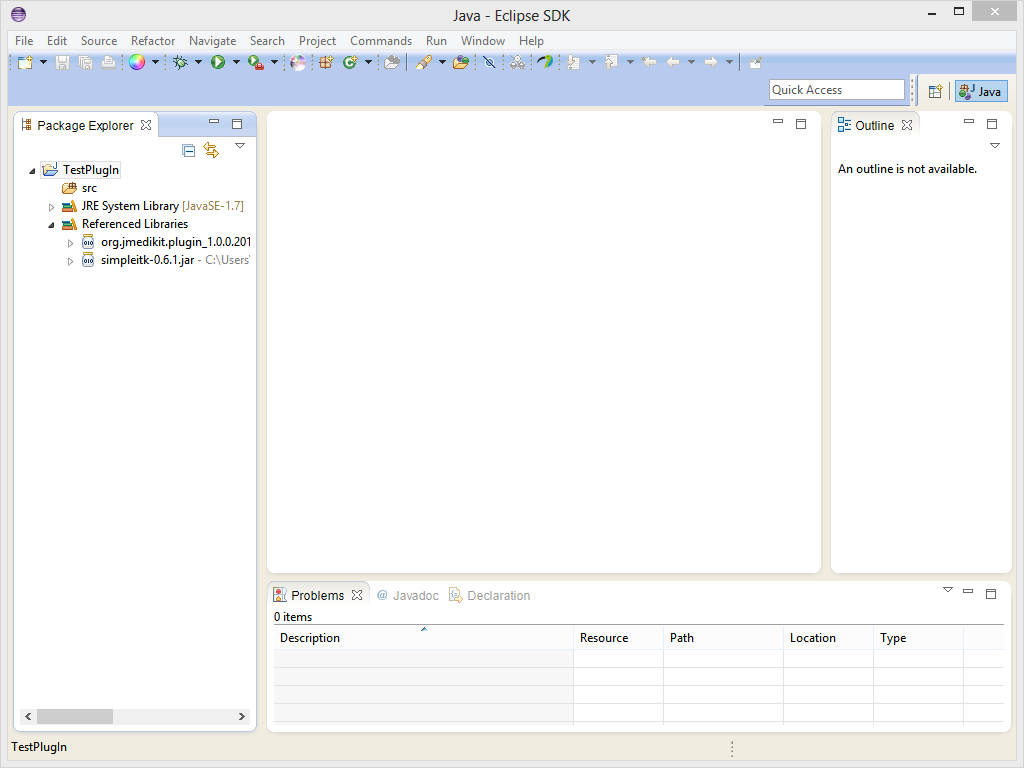
\includegraphics[angle=0,width=10cm]{./img/plugin_workspace.png}}
  \caption{Der Eclipse Workspace nach Anlegen des Projekts}
  \label{workspace}
  \vspace{0.5cm}
\end{figure}

Mit einem Rechtsklick auf den Ordner \textit{src} im Project Explorer, gefolgt von \textit{New} $\rightarrow$ \textit{Class}, kann die Hauptklasse des Plug-ins angelegt werden. Entsprechend der Plug-in-Konvetionen wird der Name \textit{\_\_TestPlugIn} mit einem Klick auf \textit{Finish} erstellt.

\begin{figure}[H]
  \vspace{0.5cm}
  \centering
  \fbox{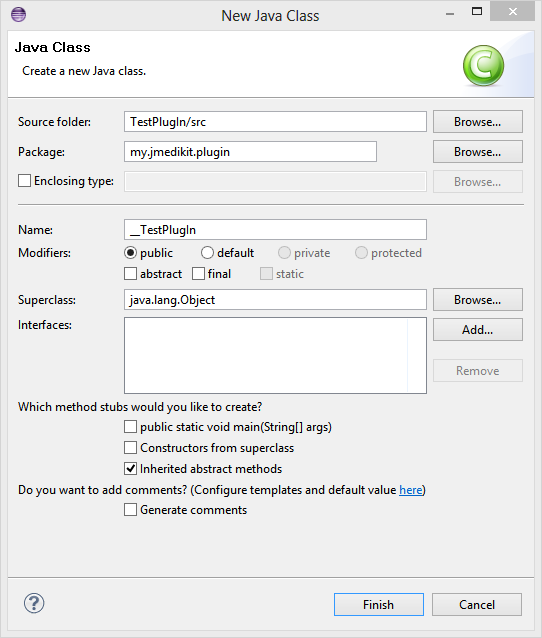
\includegraphics[angle=0,width=6cm]{./img/plugin_class.png}}
  \caption{Anlegen der Hauptklasse des Plug-ins}
  \label{class}
  \vspace{0.5cm}
\end{figure}

Nach dem Erstellen der Klasse kann mit dem Entwickeln des Plug-ins begonnen werden. Ein HalloWelt-Plug-in hat folgende Struktur:

\lstset{
language=Java,
caption={Implementierung eines HalloWelt-Plug-ins},
label=singleton,
xleftmargin=1em,
xrightmargin=1em,
numbers=left,
backgroundcolor=\color{lgrey},
}  
\begin{figure}[htbp]
\begin{lstlisting}[frame=leftline]
import org.jmedikit.lib.core.APlugIn2D;
import org.jmedikit.lib.image.AImage;


public class __TestPlugIn extends APlugIn2D{

	@Override
	public AImage process(AImage img) {
		System.out.println("Hello World");
		return img;
	}

	@Override
	protected int options() {
		setOutput("pathToOutputFile");
		return 0;
	}

}
\end{lstlisting}

\end{figure}